\section{Cluster Generation}
%1.	Visually, how does the unit contour relate to the cluster data?
The unit contour represents a collection of equally likely points in space. 
The elliptical unit standard deviation contours match the rough elliptical 
shape of the data clusters. The unit standard deviation contour does not 
enclose all data points.  This is completely expected as the random data 
points that make up the clusters were generated on a normal distribution with 
a given mean and covariance; we would not expect all data points to be within 
one standard deviation of the mean.

\section{Classification Boundaries}
%2.	Comment on the classification boundaries. How do the different boundaries
%compare?

\subsection{Parametric}

\begin{figure}
  \begin{center}
  	\label{fig:2param}  
    \caption{The clusters, unit standard deviation curves and
    parametric classification boundaries for the 2 class case.}
    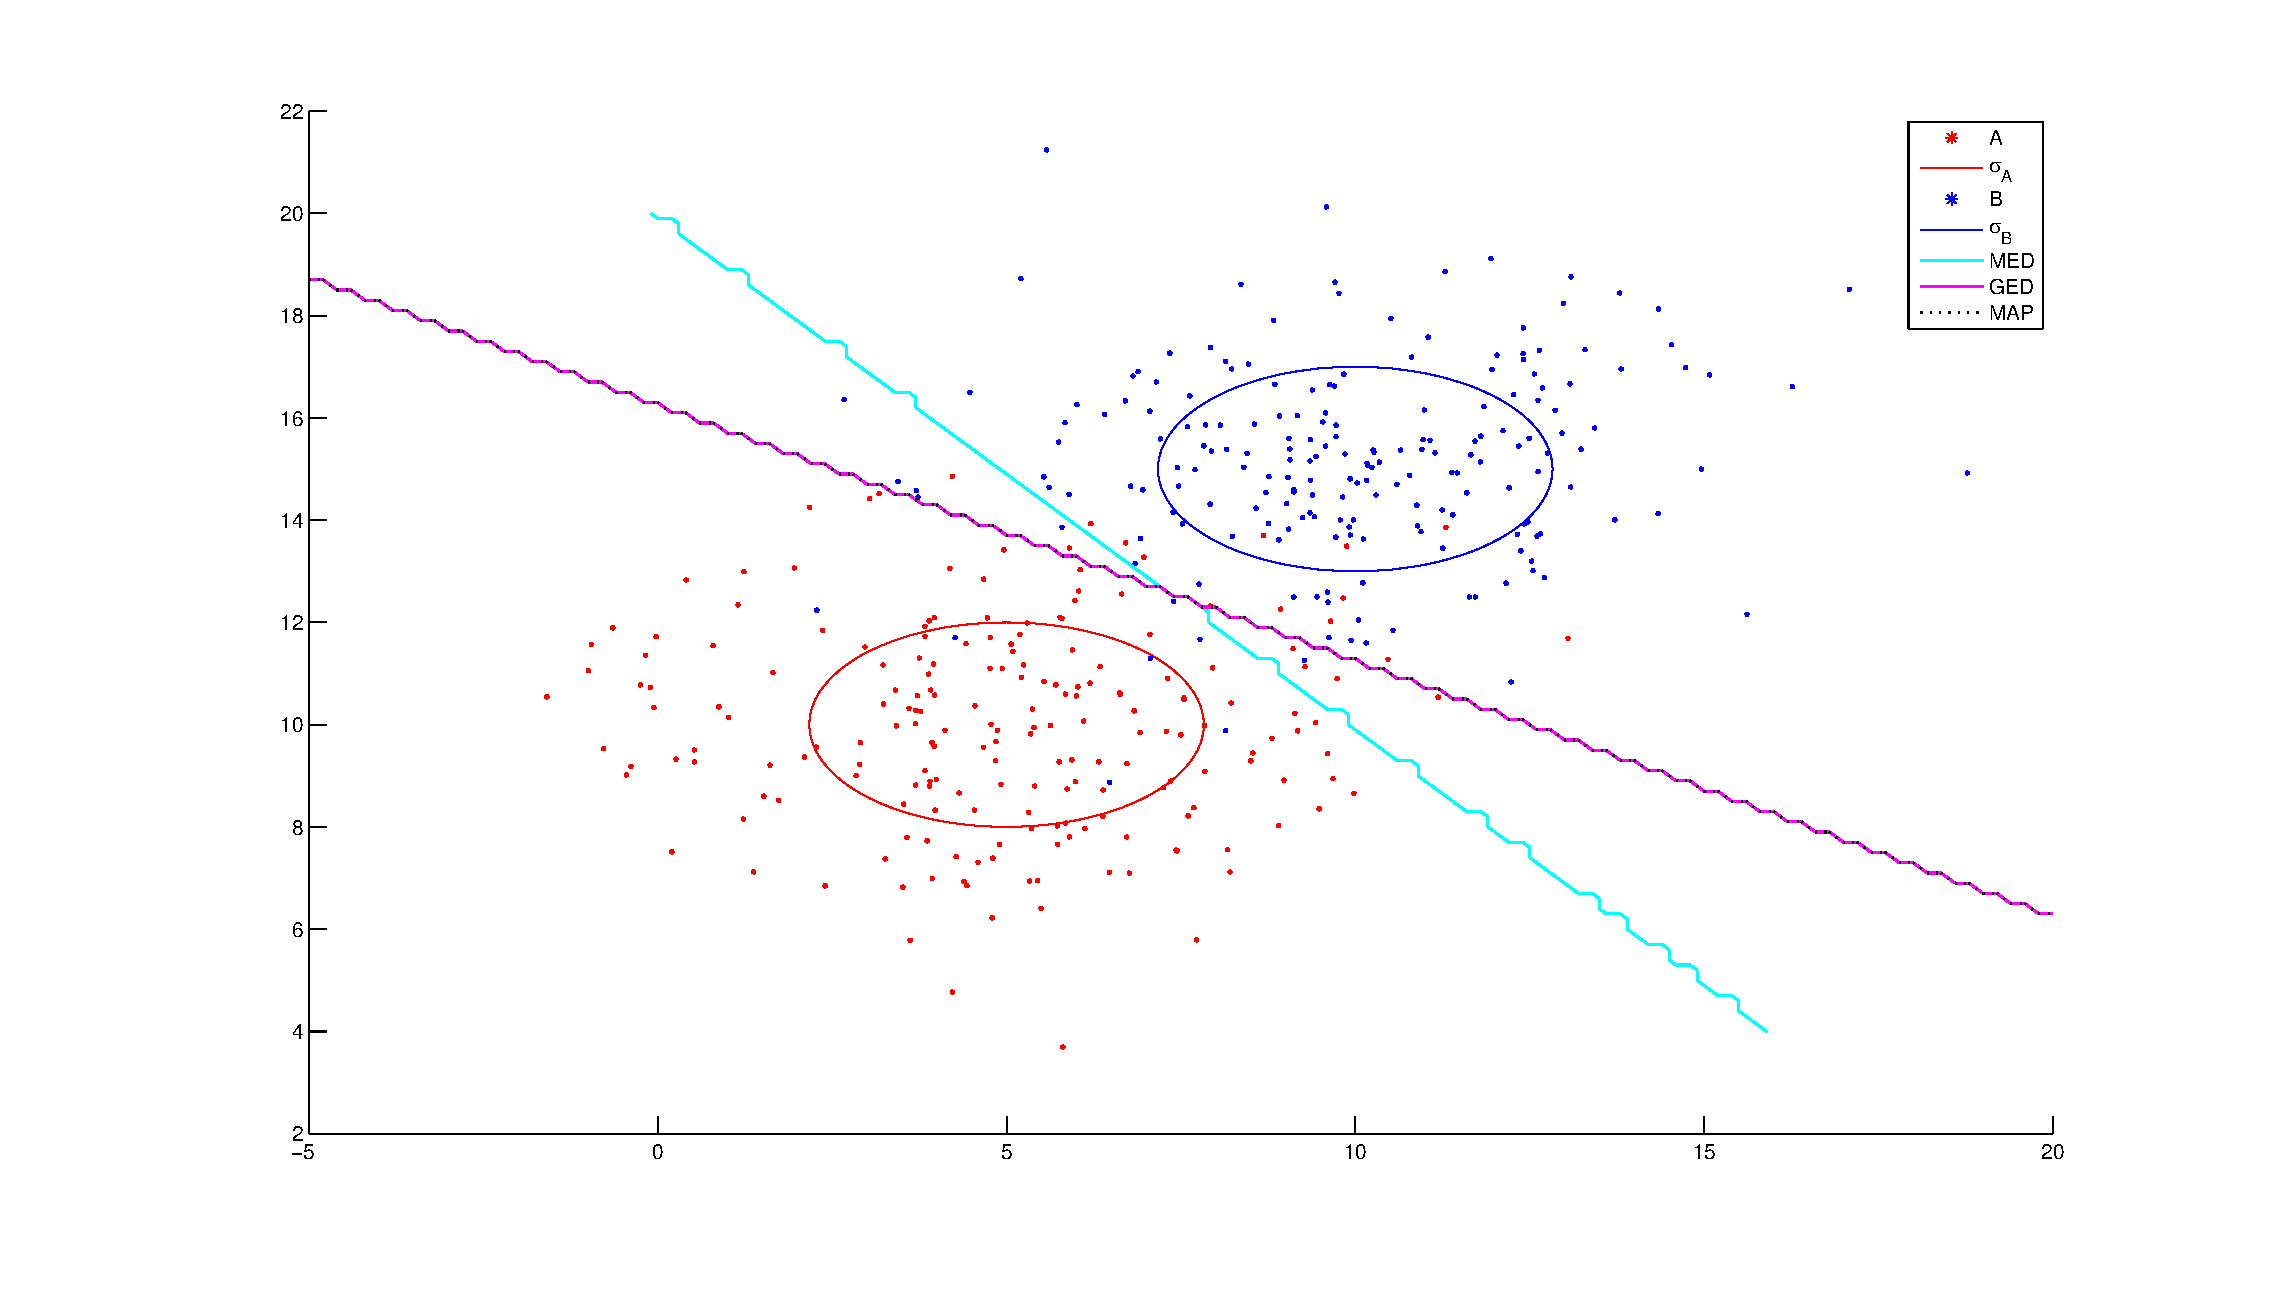
\includegraphics[width=15cm]{figures/2-param}
  \end{center}
\end{figure}

\begin{figure}
  \begin{center}
  	\label{fig:3param}
    \caption{The clusters, unit standard deviation curves and
    parametric classification boundaries for the 3 class case.}
    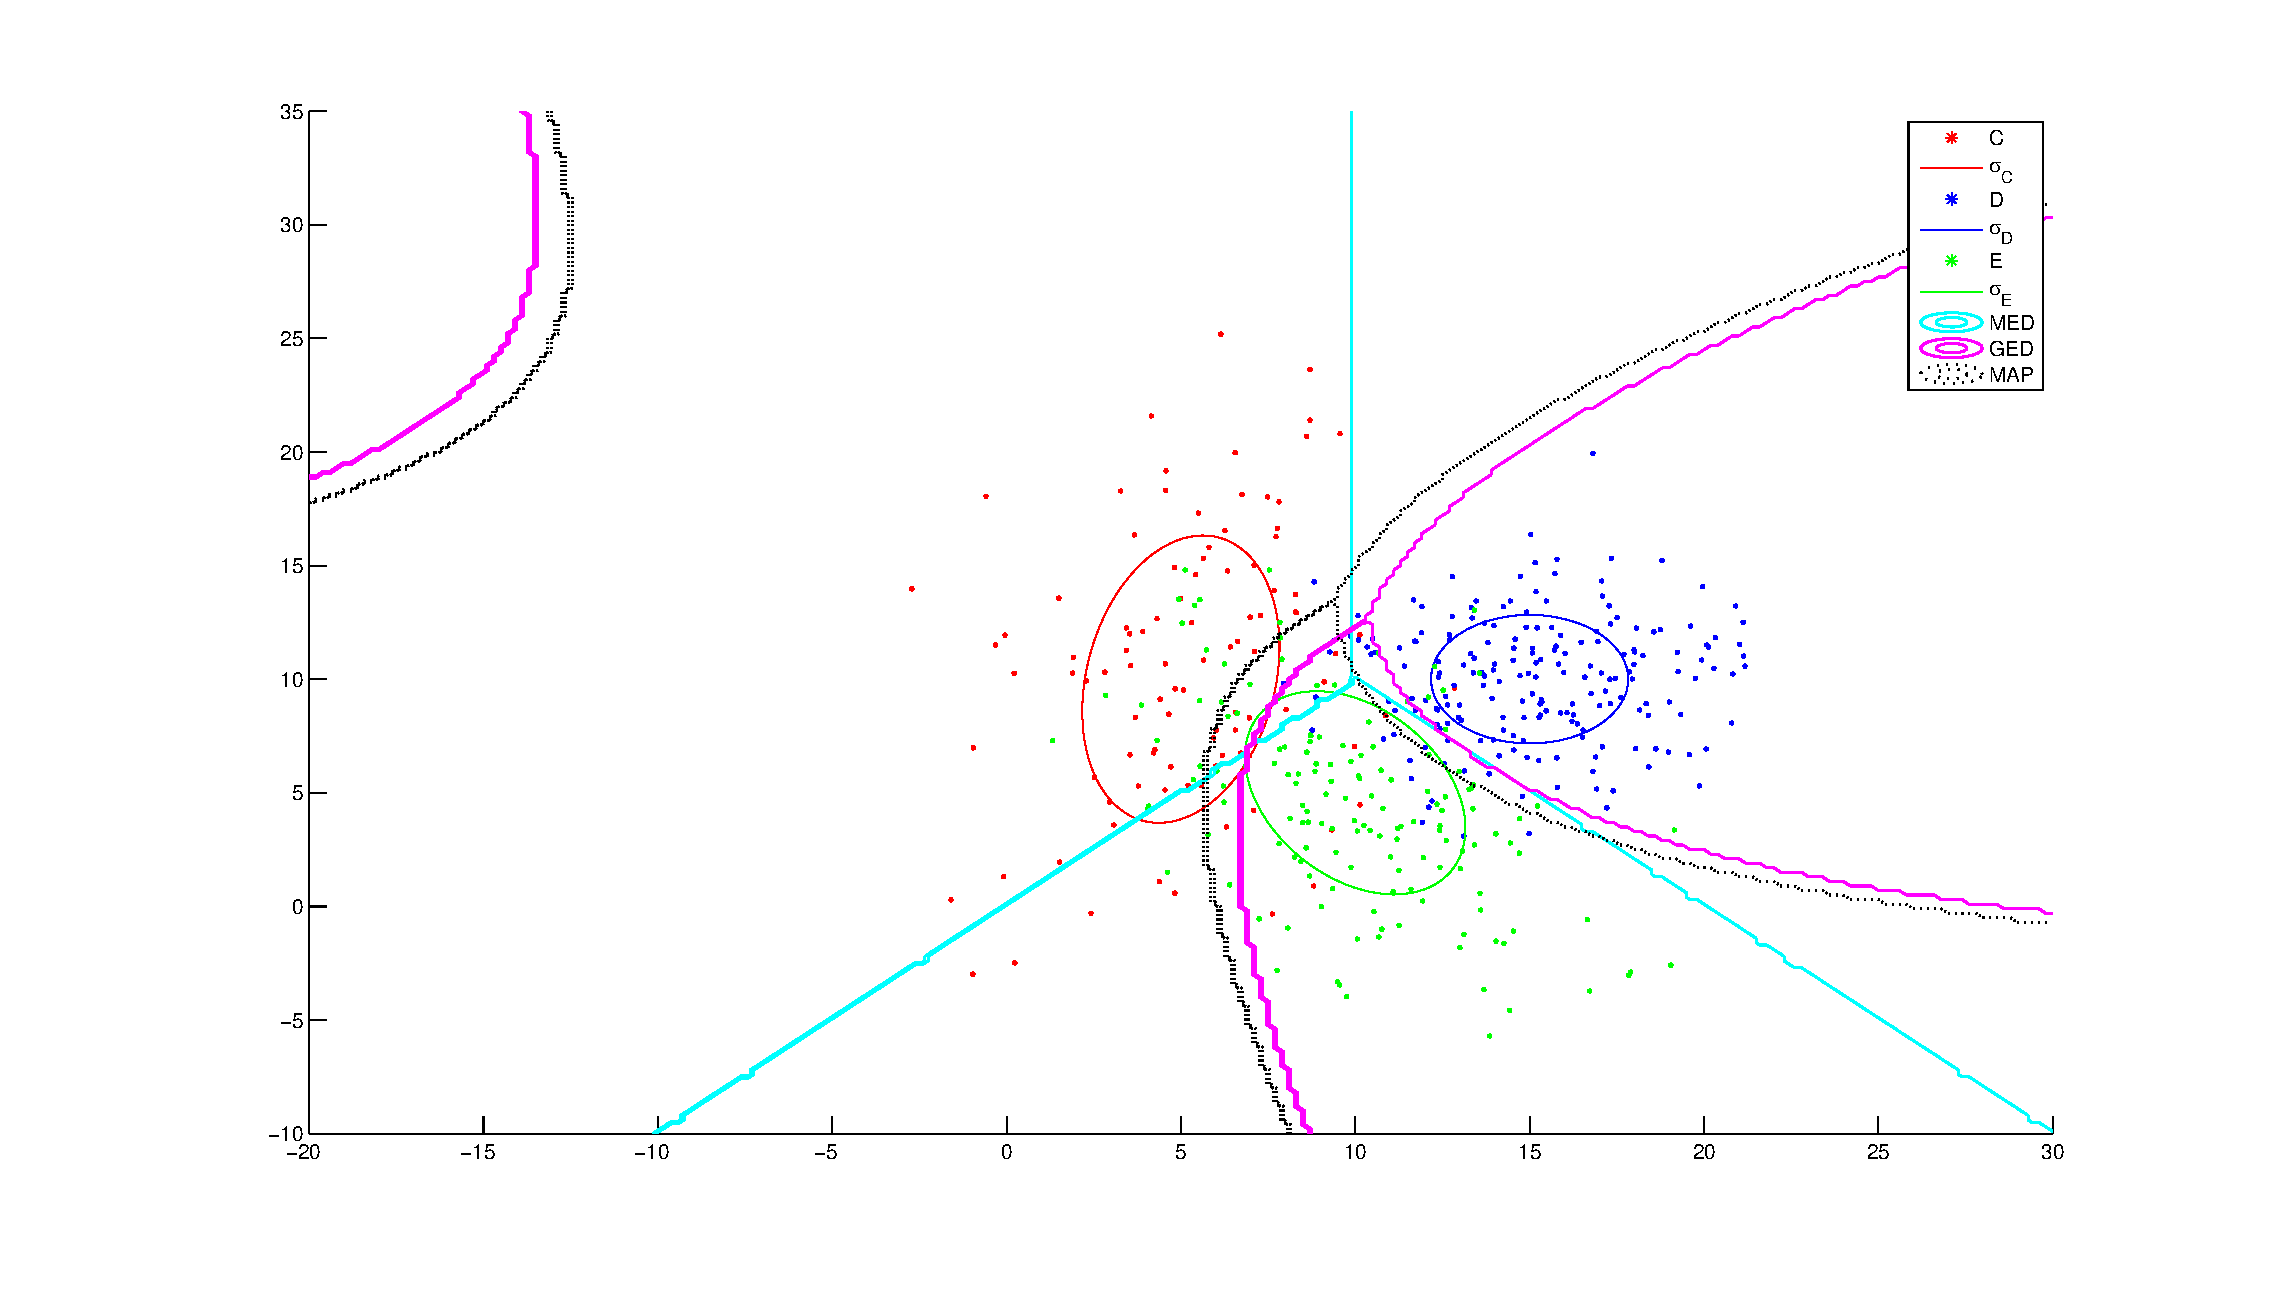
\includegraphics[width=15cm]{figures/3-param}
  \end{center}
\end{figure}

One result that was apparent in the 2-class case was that the GED classifier 
was better than MED.  The reason behind this observation is the fact that MED
does not take the shape of the cluster (ie. the variances) into account. 
Instead, MED relies solely on the location of the mean of the cluster. GED, on
the otherhand, accounts for the variances and therefore provides a more
accurate classifier, which is reflected in the lower probability of error.

This can be shown from the following observation: the MAP boundary is closer to
Class D than the GED boundary because it has a higher class probability
(Nd=200) compared with Class C (Nc=100) and E (Ne=150). For the same reason, 
compared with the GED boundary, the MAP boundary between class C and E is 
closer to Class E.

\subsection{Non-parametric}

\begin{figure}
  \begin{center}
  	\label{fig:2nonparam}  
    \caption{The clusters and non-parametric classification
    boundaries for the 2 class case.}
    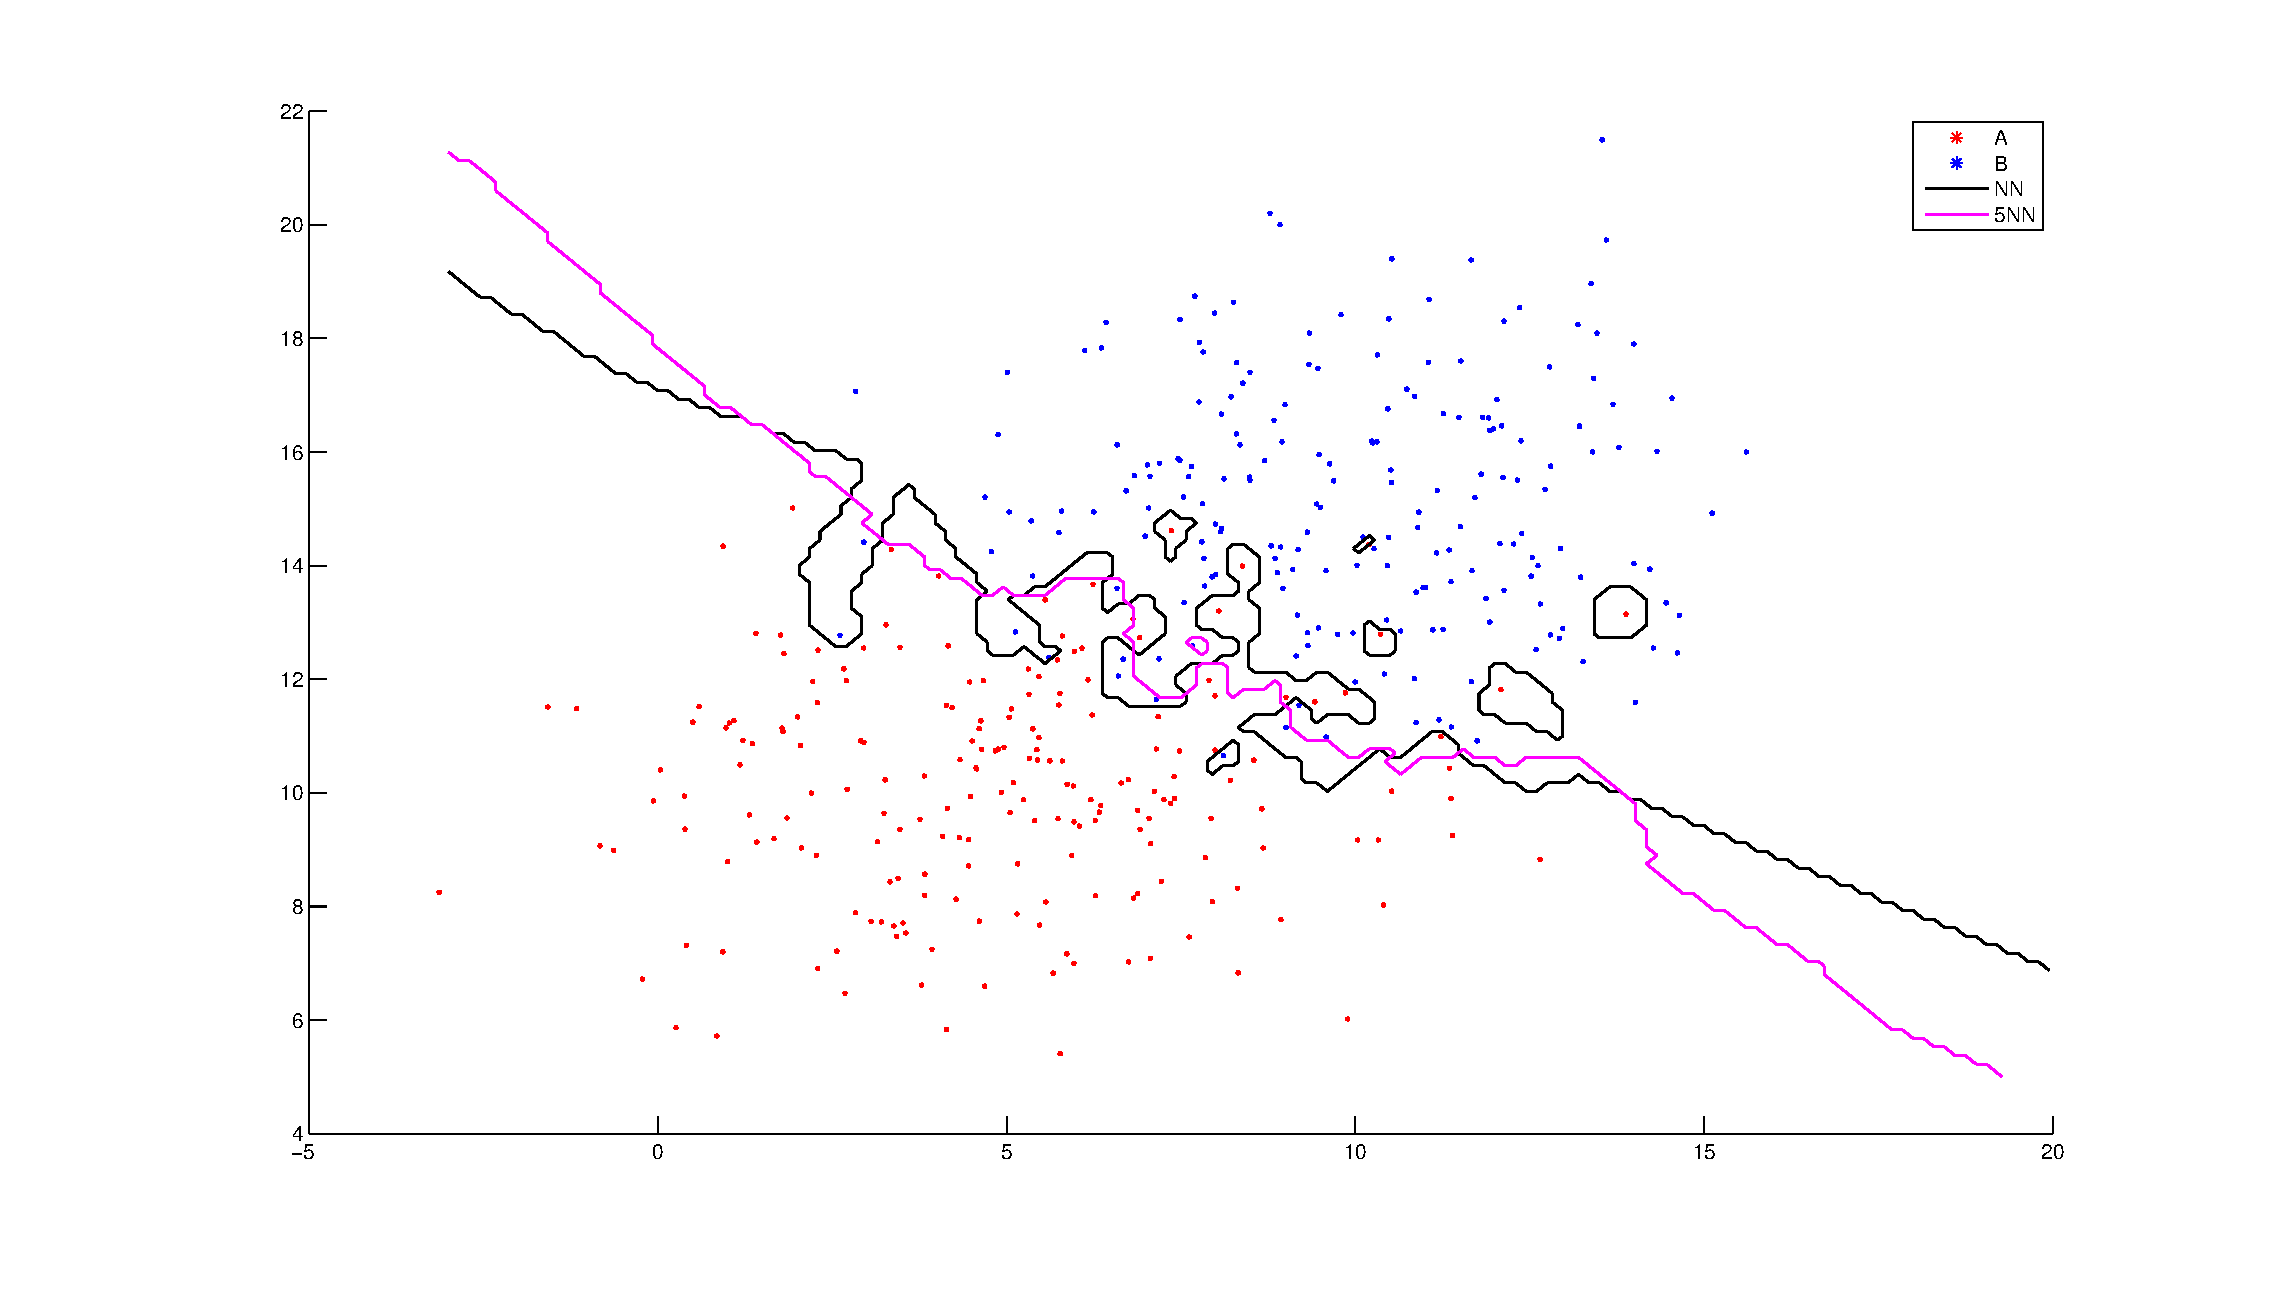
\includegraphics[width=15cm]{figures/2-nonparam}
  \end{center}
\end{figure}

\begin{figure}
  \begin{center}
  	\label{fig:3nonparam}
    \caption{The clusters and non-parametric classification
    boundaries for the 3 class case.}
    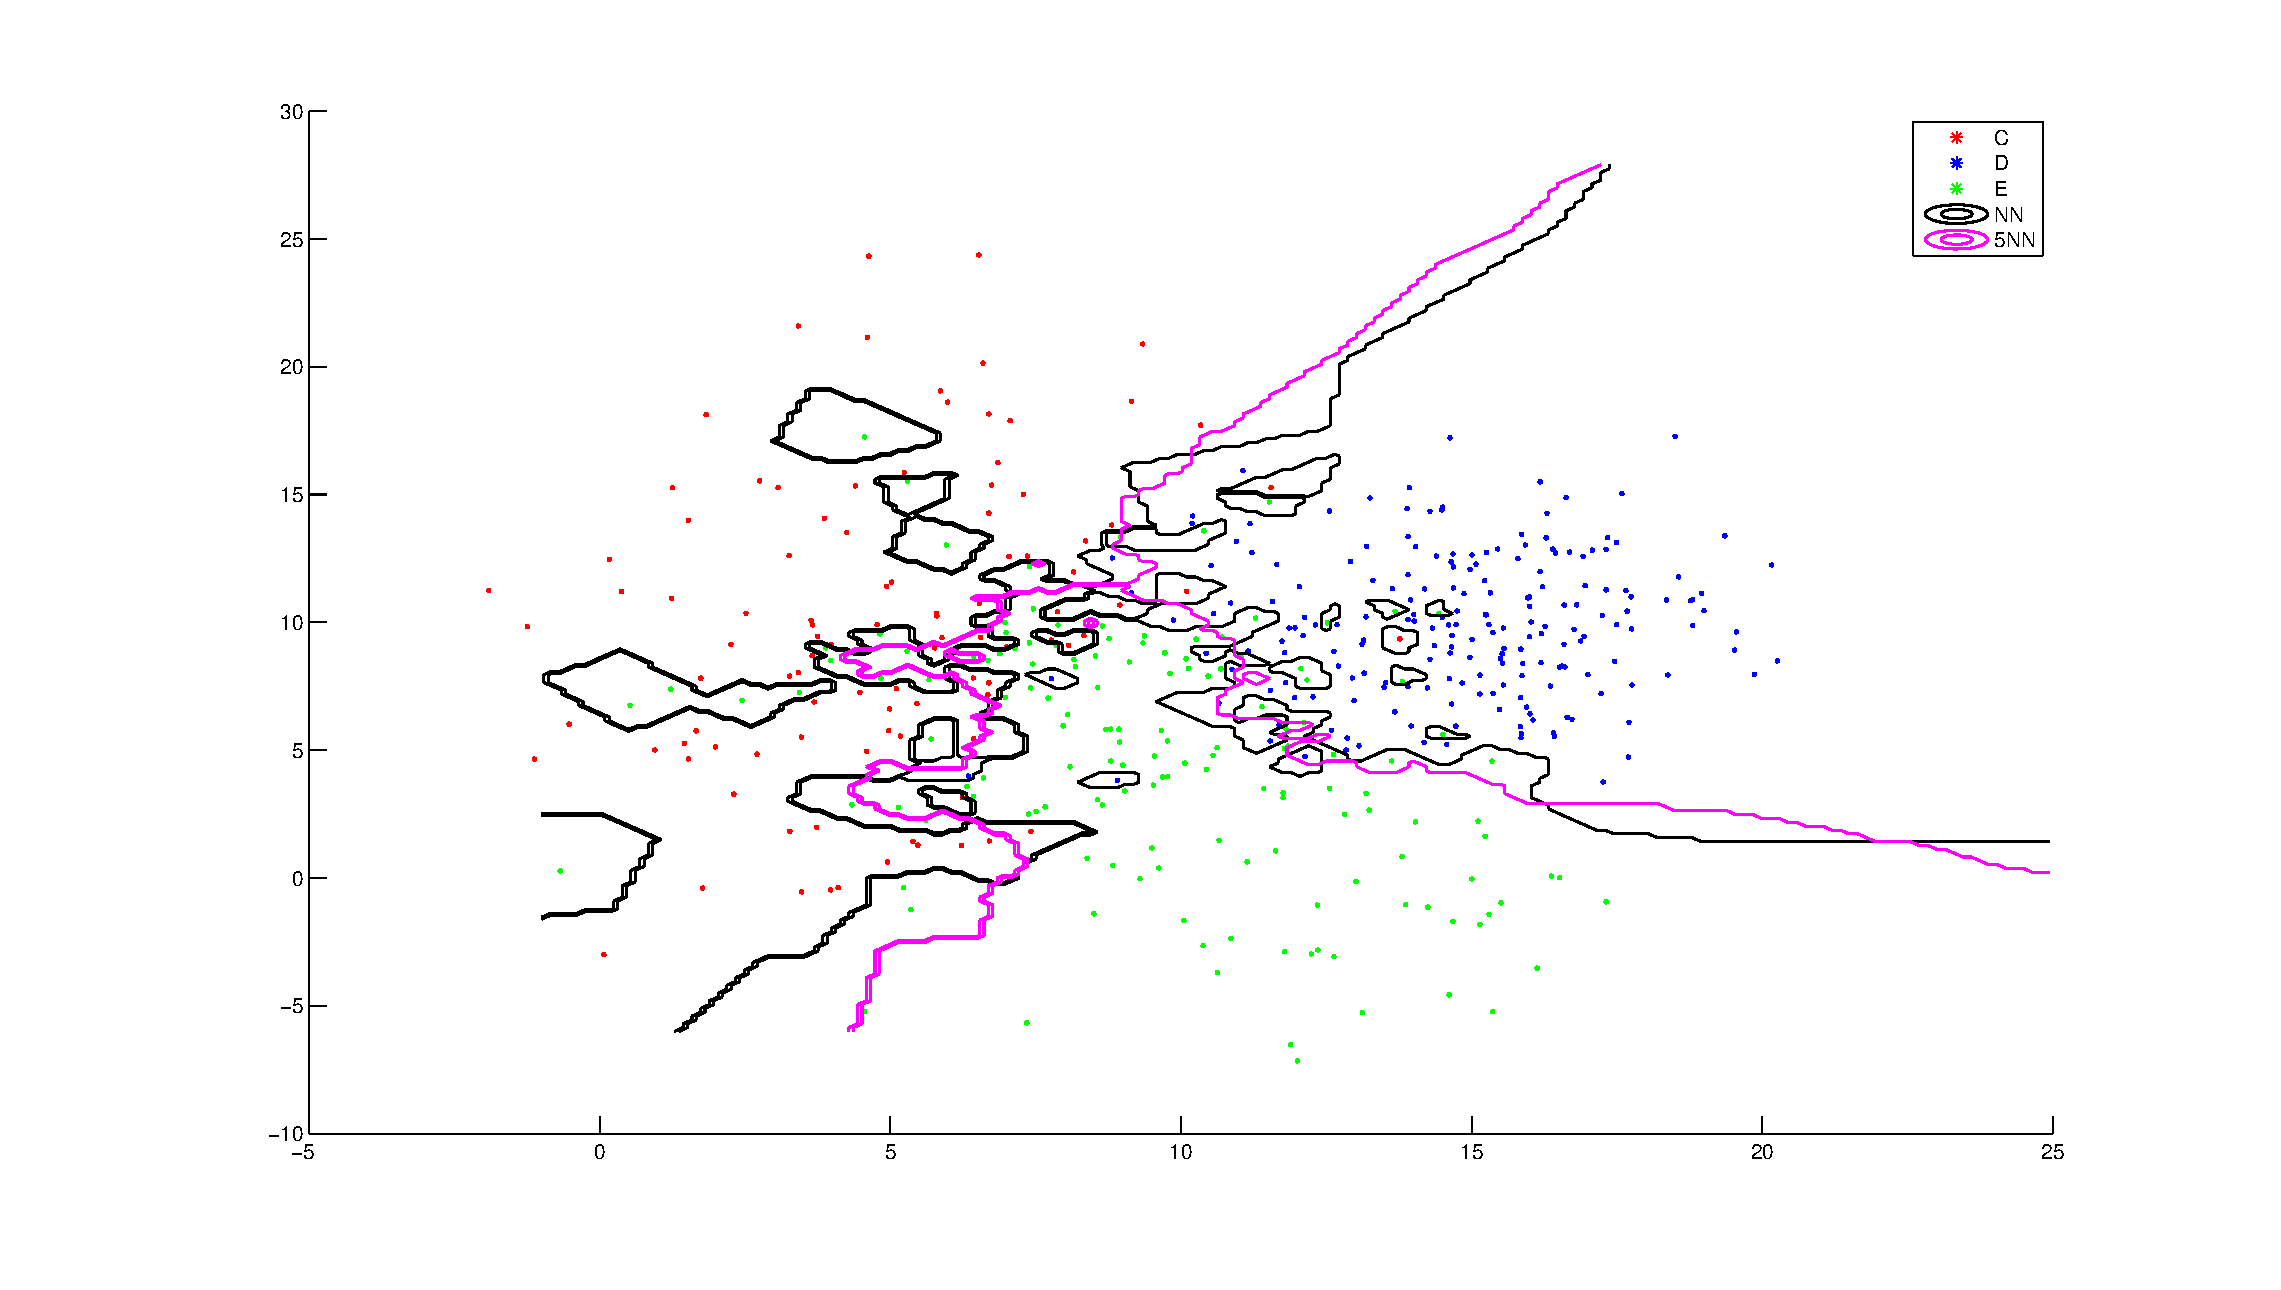
\includegraphics[width=15cm]{figures/3-nonparam}
  \end{center}
\end{figure}

Of the non-parametric classifiers, the 5NN classifier displayed a much simpler 
boundary than the NN classifier.  The key distinction is the fact that the 5NN,
by ignoring the four nearest points, is making itself much less sensitive to 
outliers. Essentially, NN differs from 5NN in two major ways. Firstly, the NN 
classifier has more individual boundaries. Secondly, these boundaries are much 
less smooth than 5NN. However, NN both runs faster and requires less memory 
since it does not demand the sorting of the distances from the testing points 
to all the training data.

\section{Error Anaylsis}
%3.	Compare the results. Which error is smallest? What do you observe in the
%confusion matrices for CASE2?

\begin{table}[h]
\centering
\caption{Confusion matrix and probability of error for the 2 class case}
\label{tab:conf2class}
\vspace{6pt}
\begin{tabular}{lcc}
\toprule
Classification Method & $M_{confusion}$ & $P(\varepsilon)$ \\
\midrule
MED &
\begin{bmatrix}
188 & 15 \\
12  & 185 \\
\end{bmatrix}
& 62.86 \\
GED & 28.93	& 28.21	\\
MAP & 46.43	& 8.57	\\		
\midrule
\midrule
Total domestic energy (\%) & 4.51	& 4.62	& 4.76	& 4.63 \\
\bottomrule
\end{tabular}
\end{table}

In the first case, the covariance matrices of both classes were identical,
driving the MAP classifier to be identical to the GED classifier.  This result
is supported by a simple consideration of the additional terms in MAP that 
differentiate it from GED.  The classes are equally likely, so $\ln(\Theta)$
goes to zero.  Also, the classes have the same covariance matrix, resulting in the
$\ln(\Sigma)$ terms cancelling out to zero.  This leaves the exact GED
formula, thus confirming the observed result.  In the three class case, the three
classes are not equally likely and therefore MAP provides a better classifier. 
MAP prefers classes that are more compact and have a higher probability density
in a given region. From these observations, it can be gathered that, if the two
classes have the same covariance and if both means fall on the line drawn by
the  axes of the other class, then MED, GED and MAP will all be the identical 
(and they will in fact be right bisectors).

For the non-parametric case, K-NN has smaller error than NN. This is again
attributed to the fact that the former is less sensitive to outliers in the 
training data. It is observed from the confusion matrices that the elements in
(1, 2) and (2, 1) are much smaller than the rest of the off-diagonal elements. 
This provides a good indication that Class C and D probably have comparitively 
very little overlap with each other.  Observations such as this can provide
some intuition about the location of the classes simply from seeing an error analysis.

In the first case, MAP does better than K-NN. However, it is the other way
around for the second case. Therefore, the relative performances of parametric 
and non-parametric classifiers are case-based even when the assumption for the 
shape of the class holds.

To explore the effect of the choice of k on the probability of error, a simple 
for loop was created to calculate the probability of error for the range 
of possible k ($0 < k < n_{smallest\_class}$).  This generally
showed a sharp decrease initially, as outliers are ignored.  After the initial drop, 
the graphs behave slightly differently for the 2- and 3-class cases.  For the 
2-class case, we found that the probability of error remains fairly flat for
the majority of the values of k, with a spike as k approaches its maximum
value. For the 3-class case, however, it seems that the probability of error 
begins to climb again immediately following the initial drop.  This suggests 
that class structure is eroded more quickly due to the exclusion of good data 
for the 3-class case.  From this result, we might suspect that this trend would
hold as the number of classes increases.
